%\documentclass[letterpaper,10pt, jcp, aps]{revtex4-1}
\documentclass[superscriptaddress,pre,reprint,showpacs,twocolumn]{revtex4-1}

\usepackage[utf8]{inputenc}
\usepackage{amsmath, amsfonts}
\usepackage{graphicx}
\usepackage{natbib}
\usepackage{caption}
\usepackage{subcaption}
%\usepackage{authblk} parece ser que ya esta metido cuando usas preprint

\usepackage{hyperref}


%\bibliographystyle{alpha}

%opening

%\author{Rosa Rodríguez \& David P.~Sanders \& W. P. K. Zapfe}
%\affil{Departamento de Física, Facultad de Ciencias, Universidad Nacional Autónoma de México, Ciudad Universitaria, Del.~Coyoacán, México D.F. 04510, Mexico}

\usepackage{mathptmx}
% I dont know if that package is compatible with revtex.

\newcommand{\defeq}{:=}
\newcommand{\mean}[1]{\left \langle #1 \right \rangle}
\newcommand{\rd}[1]{\mathrm{d}{#1} \,}
\newcommand{\RR}{\mathbb{R}}
\newcommand{\vv}{\mathbf{v}}
\newcommand{\indicatorsymbol}{\mathbf{1}}
\newcommand{\indicator}[1]{\indicatorsymbol_{ \{   #1 \} } } 
\newcommand{\etal}{et al.\ } 

\setlength{\parskip}{10pt}
\setlength{\parindent}{0pt}


\begin{document}

\title{Exact hopping and collision times for two hard discs in a box}

\author{Rosa Rodríguez}
\email{rosarm@physics.mcgill.ca}
\affiliation{Physics Department, McGill University}

\author{David P.~Sanders}
\email{dpsanders@ciencias.unam.mx}
\affiliation{Departamento de Física, Facultad de Ciencias, Universidad Nacional Autónoma de México, Ciudad Universitaria, Ciudad de México 04510, Mexico}

\author{W.~P.~Karel Zapfe}
\email{karelz@cinvestav.mx}
\affiliation{Departamento de Física, Facultad de Ciencias, Universidad Nacional Autónoma de México, Ciudad Universitaria, Ciudad de México 04510, Mexico}

\affiliation{CINVESTAV-IPN, Mexico}


\begin{abstract}
We study the molecular dynamics of two discs undergoing hard collisions in a rectangular box.
Using a mapping to a billiard model and a key result from ergodic theory, we obtain exact expressions for mean times between different classes of events:
hops, i.e. horizontal or vertical interchanges of the particles; wall collisions; and disc collisions.
To do so, we calculate
volumes and cross-sectional areas in the four-dimensional configuration space.
In all cases, we compare exact analytical results against Monte Carlo simulations, with excellent agreement.
\end{abstract}

\maketitle



\section{Introduction}

%\typeout{`` this is ``  \the\columnwidth }

Collision times play a fundamental role in statistical mechanics, since properties
such as mixing, reaction and diffusion rates depend on them \cite{Boltz72, Tolman, VanKampen}.
A paradigmatic model, introduced by Boltzmann almost 150 years ago \cite{Boltz72, SzaszBook00},
consists of a fluid of hard spheres colliding with one other, either in a periodic torus or in
a rectangular box.

The simplest such system that is non-trivial is that of two discs in a box.
The discs move rectilinearly until they undergo
elastic collisions, either with a wall of the box, or with one another; this has been called ``inertial motion'', to distinguish it from Brownian motion \cite{Bowles04}.
Phenomena such as transport, collision and reaction
have been studied in this systems, both analytically 
 \cite{Awazu01, Munakata02, Suh05} and numerically \cite{MacElroy2004, MacElroy2005}.
 Events of physical interest in this system are \emph{hopping},
in which two particles interchange position, either vertically or horizontally,
and \emph{collisions} of the particles, with the box or with one other. Hopping plays an important role in the dynamics of confined fluids, for example
REF.

 
Previous work
by Bowles \etal gives general quantitative results for hopping times 
for both inertial and Brownian dynamics \cite{Bowles04}. They focus
on the mean \emph{first-passage} time, using arguments from transition state theory 
to provide expressions for the general behavior of these quantities, as a function of the
disc radii. %Their results show the adequate algebraic behavior.
Further work has expanded along that line  \cite{Suh05, Ball09}.
There is also a statistical thermodynamic treatment by Munakata \etal, 
who study the partition function, pressure,
and temperature in the system \cite{Munakata02, Munakata06}. 


In this paper we obtain \emph{exact} analytical expressions, not for the first passage time,
but rather for mean inter-hop and inter-collision times of two discs under 
inertial (Newtonian) motion, as a function of the geometrical parameters of the system. Such a treatment is possible
 since the dynamics of $N$ hard discs in $d$ spatial dimensions
 is equivalent to a \emph{billiard model} in the $Nd$-dimensional configuration space, i.e. a \emph{single} point particle colliding elastically 
with suitable objects (``scatterers'') \cite{SzaszBook00}. 
In particular, the system of two discs in a box is hyperbolic (chaotic) and ergodic when the discs are able to pass each other \cite{Sim99}. Otherwise, the system decomposes itself into
a finite number of disjoint ergodic components (two or four), which are each still hyperbolic.

We can thus apply a key result from ergodic theory on mean collision times \cite{Chernov97} to obtain analytical expressions 
for times between hops, between wall collisions, and between disc collisions; these are verified numerically. 
%The difficulty in the calculations lies in correctly accounting for various
%factors occurring in the expressions. 
In certain asymptotic regimes, we recover previously obtained power-law exponents \cite{Bowles04}.

The main difficulty in the analysis is correctly accounting for several geometric factors with different origins in both the
analytical and numerical calculations.

%The previous  results on
%inertial dynamics can be extended  by particularizing 
%exact expressions for the mean return times (MRT). 
%We shall  obtain them through application of 
%Machta and Zwanzig formula for residence times \cite{MachtaZwan} ??
%We shall also  compare \emph{mean event times} with 
%\emph{mean first event times} (MFET),
%and give some arguments to explain the agreement between the two. 
%Brownian dynamics shall be discussed elsewhere \cite{WorkInProgress}.
%We shall also provide this paper with supplementary material 
%detailing the calculations. 



\section{Model: Two hard discs in a rectangular box}

We consider two hard discs with equal radius $r$,
moving inside a box of width $w$ and height $h$; see Fig.~\ref{billar01}. 
The discs move inertially in the absence of forces, 
following straight line trajectories,
and undergo elastic collisions with one 
other and with the walls of the box.

\begin{figure}[h]
  \begin{center}
    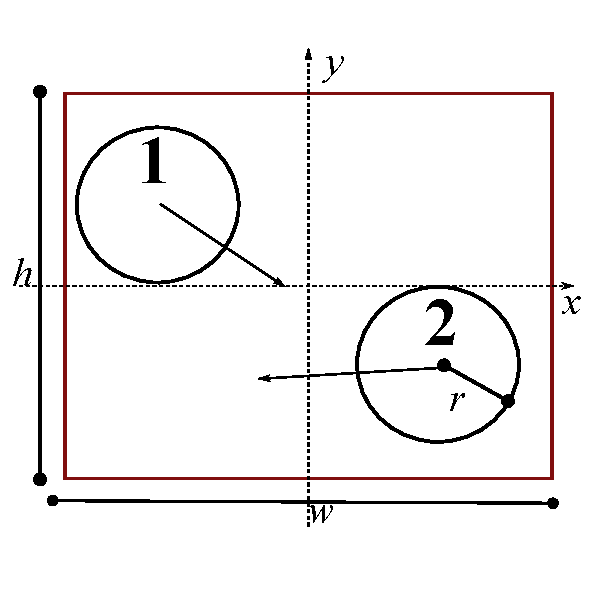
\includegraphics[width=0.40\textwidth]{figures/DiscsBox01.pdf}
  \end{center}
  \caption{The billiard and its parameters. Coordinates
    have their origin at the geometrical center of the 
    billiard table.}\label{billar01}
\end{figure}


We denote the position of the center of the $i$th disc by 
$\mathbf{x}_i = (x_i, y_i)$, and its velocity by $\mathbf{v}_i = (u_i, v_i)$ for $i=1,2$. Since the discs are hard, 
their centers are restricted to the region 
$(x_i, y_i) \in [-a,a] \times [-b, b]$, where 
$a \defeq a(r) \defeq \frac{w}{2} - r $ and
$b \defeq b(r) \defeq \frac{h}{2} - r $.

The exclusion condition preventing the discs from overlapping is $(x_1-x_2)^2 + (y_1-y_2)^2 \ge (2r)^2$.
It is thus useful to perform an orthogonal transformation (rotation) to the following new coordinates:
\begin{equation}\label{cambiocoor01}
  \begin{split}
 x  \defeq \frac{x_1 - x_2}{\sqrt{2}};  &
\quad X  \defeq \frac{x_1 + x_2}{\sqrt{2}};  \\
 y  \defeq \frac{y_1 - y_2}{\sqrt{2}}; & 
\quad Y  \defeq \frac{y_1 + y_2}{\sqrt{2}}.
\end{split}
\end{equation}


In these coordinates, the configuration space is given by the following
intervals:
$x \in [-a \sqrt{2}, +a \sqrt{2}]$ with 
$X \in [-a \sqrt{2} + |x|, a \sqrt{2} - |x|]$; and similarly for $y$ and $Y$, replacing $a$ by $b$.
The non-overlapping constraint becomes $x^2 + y^2 \ge 2 r^2$.
The horizontal and vertical coordinates transform independently
from each other, and the Jacobian of this transformation is  equal to $1$.

These constraints define a four-dimensional
rectangular prism, in which is embedded an excluded cylinder with a three-dimensional surface
(codimension 1).
This cylinder has radius $r\sqrt{2}$ and lies
on a diagonal between the $X$ and $Y$ axes.
The prism surface is the outer boundary of the configuration space,
while the cylinder is an excluded volume, the surface of which
acts as a reflecting inner boundary.
The dynamics of the two discs is equivalent to a billiard model in this 4-dimensional space, in which 
a point particle undergoes free flight until
it hits a wall, where it undergoes an elastic reflection.
The outer boundaries are flat, so the
hyperbolicity is due to the inner semi-dispersing
boundary \cite{Sim99}, which corresponds to the collision of
the two discs.


We take the mass of each disk as $m=1$, so that the kinetic energy
is $\frac{1}{2}(\mathbf{v}_1^2 + \mathbf{v}_2^2)$. We restrict attention to the energy surface with
$E = \frac{1}{2}$, so that the disc velocities satisfy $\mathbf{v}_1^2 + \mathbf{v}_2^2 = 1$.
Other values of the mass or energy correspond to a simple rescaling of the dynamics, with velocities differing
by a factor of
$\sqrt{2E/m}$, and corresponding factors in the times to be determined below.


\section{Mean collision time for billiard models}

\label{knownfacts}
%\subsection{Known facts on collision rates}

A system of $N$ hard spheres confined by hard walls in a $d$-dimensional
space may be treated as a billiard system 
in which a single point particle undergoes free motion between reflecting obstacles 
in a $ (d N) $-dimensional configuration space \cite{Sinai70, Sim99, MarkChern}. 
%If the resulting billiard is ergodic and hyperbolic, then we know that
%these systems are equivalent to Bernoulli flows \cite{Gallavotti74}.
This can be thought of as a mean return time to the $(d-1)$-dimensional 
(i.e. co-dimension $1$) cross-section given by the wall boundaries.

For a particle with unit velocity moving in a general billiard table, there is 
an exact expression for the mean time between 
collisions of the particle with a given wall \cite{Chernov97}:

\begin{equation}\label{meanfreetime}
 \mean{\tau} = \frac{|Q|}{|A|} \cdot \frac{|S^{d-1}|} {|B^{d-1}|} \cdot \frac{1}{s}.
\end{equation}


Here, $|Q|$ denotes the $d$-dimensional volume of the available 
space in the billiard and 
$|A|$ the $(d-1)$-dimensional area of the cross-section.
 $|S^{d-1}|$ is the $(d-1)$-dimensional area of the unit sphere in $\RR^d$, given by
\begin{equation}
  |S^{d-1}| = \frac{2 \pi^{d/2}}{\Gamma(d/2)},
\end{equation}
where $\Gamma(\cdot)$ is the gamma function. 
$|B^{d-1}|$ is the volume of the unit ball 
in $\RR^{d-1}$, given by $|B^{d-1}| = |S^{d-2}| / (d-1)$.
The extra factor $1/s$ involves the ``sidedness'' factor, explained below.
Note that Machta and Zwanzig \cite{MachtaZwan} used a similar method to derive an escape 
time across a virtual boundary by treating it as a recurrence time.
%Since it is an escape time, they used velocities whose components point only 
%perpendicularly to the ``exit wall''.

In our case, we are interested in the mean return time to 
several types of co-dimension-$1$ cross section.
The first, giving the ``hopping time'', 
is defined by the moment
at which the discs interchange their horizontal or vertical position, i.e.
when they cross one of the two surfaces
\begin{equation} \label{condchoque}
x_1 = x_2  \qquad \text{or} \qquad y_1 = y_2.
\end{equation}
At such an event, the cross-section can be hit from \emph{either} side,
e.g., the disk 1 can be traveling from left to right or the other way around
at the moment when the interchange of positions take place. 
The area $A$ of the surface is, then, 
effectively twice as large; this will be given by a ``sidedness'' factor $s=2$ in the formula
for $\mean{\tau}$.

The other events of interest correspond to collisions of a specific
disc with a specific wall, and the mutual collision between the two discs.
In both of these cases, the collision surface can be reached only from one side, corresponding to $s = 1$.

To calculate the mean times of interest, it is thus necessary to calculate
the 4-dimensional volume $V$ of the available space, and the 3-dimensional cross-sectional area $A$ 
for each event of interest. The main difficulty consists of correctly accounting for multiplicative factors associated to the different 
types of areas.



\section{Calculation of volume and areas}

%The configuration
%space is an four dimensional prism with a four dimensional
%cylinder subtracted.
%The calculation can be carried out indirectly,
% using indicator functions for the
%available space or for the prohibited space.

\subsection{Volume of available space}

%%%% Esta linea me confunde, no entiendo del todo a que se refiere "the complement of the cylinder in the configuration space",
%%%% y se podria evitar el where where
We denote by $Z := \{ \mathbf{x} \in \mathbb{R}^4: (x_1-x_2)^2 + (y_1-y_2)^2 \ge (2r)^2 \}$, where
the complement of the cylinder in the configuration space, where $\mathbf{x} := (x_1, x_2, y_1, y_2)$.
The four-dimensional available volume $V_\text{free}$ is then given by
\begin{align}\label{volindic}
V_\text{free} &= 
\iiiint
\limits_{\substack{x_1, x_2 = -a \\ y_1, y_2 = -b}}^{\substack{x_1, x_2 = a \\ y_1, y_2 = b}}
\rd x_1 \rd x_2 \rd y_1 \rd y_2 
\, \indicator{ (x_1-x_2)^2 + (y_1-y_2)^2 \ge (2r)^2 } \\
&=
\int  \mathrm{d} \mathbf{x} \, \indicatorsymbol_Z(\mathbf{x}), 
\end{align}
where $\int  \mathrm{d} \mathbf{x}$
%$$ \int  \mathrm{d} \mathbf{x} :=  \int_{x_1 = -a}^a \rd x_1  \int_{x_2 = -a}^a \rd x_2
%\int_{y_1 = -b}^b \rd y_1 \int_{y_2 = -b}^b  \rd y_2 $$
denotes a four-dimensional integral over the whole volume, and 
$\indicatorsymbol_Z$ is the indicator function of the set $Z$, 
given by $\indicatorsymbol_Z (\mathbf{x}) = 1$ if $\mathbf{x} \in Z$, and $=0$ if $\mathbf{x} \notin Z$.
Fig.~\ref{diagintegral01} shows a diagram of the product of
spaces that give rise to the whole configuration space.
Recall that the dimensions $a$ and $b$ of the available configuration space are functions of the disc radius $r$, 
but we suppress this explicit dependence for simplicity.

\begin{figure}[h]
  \begin{center}
    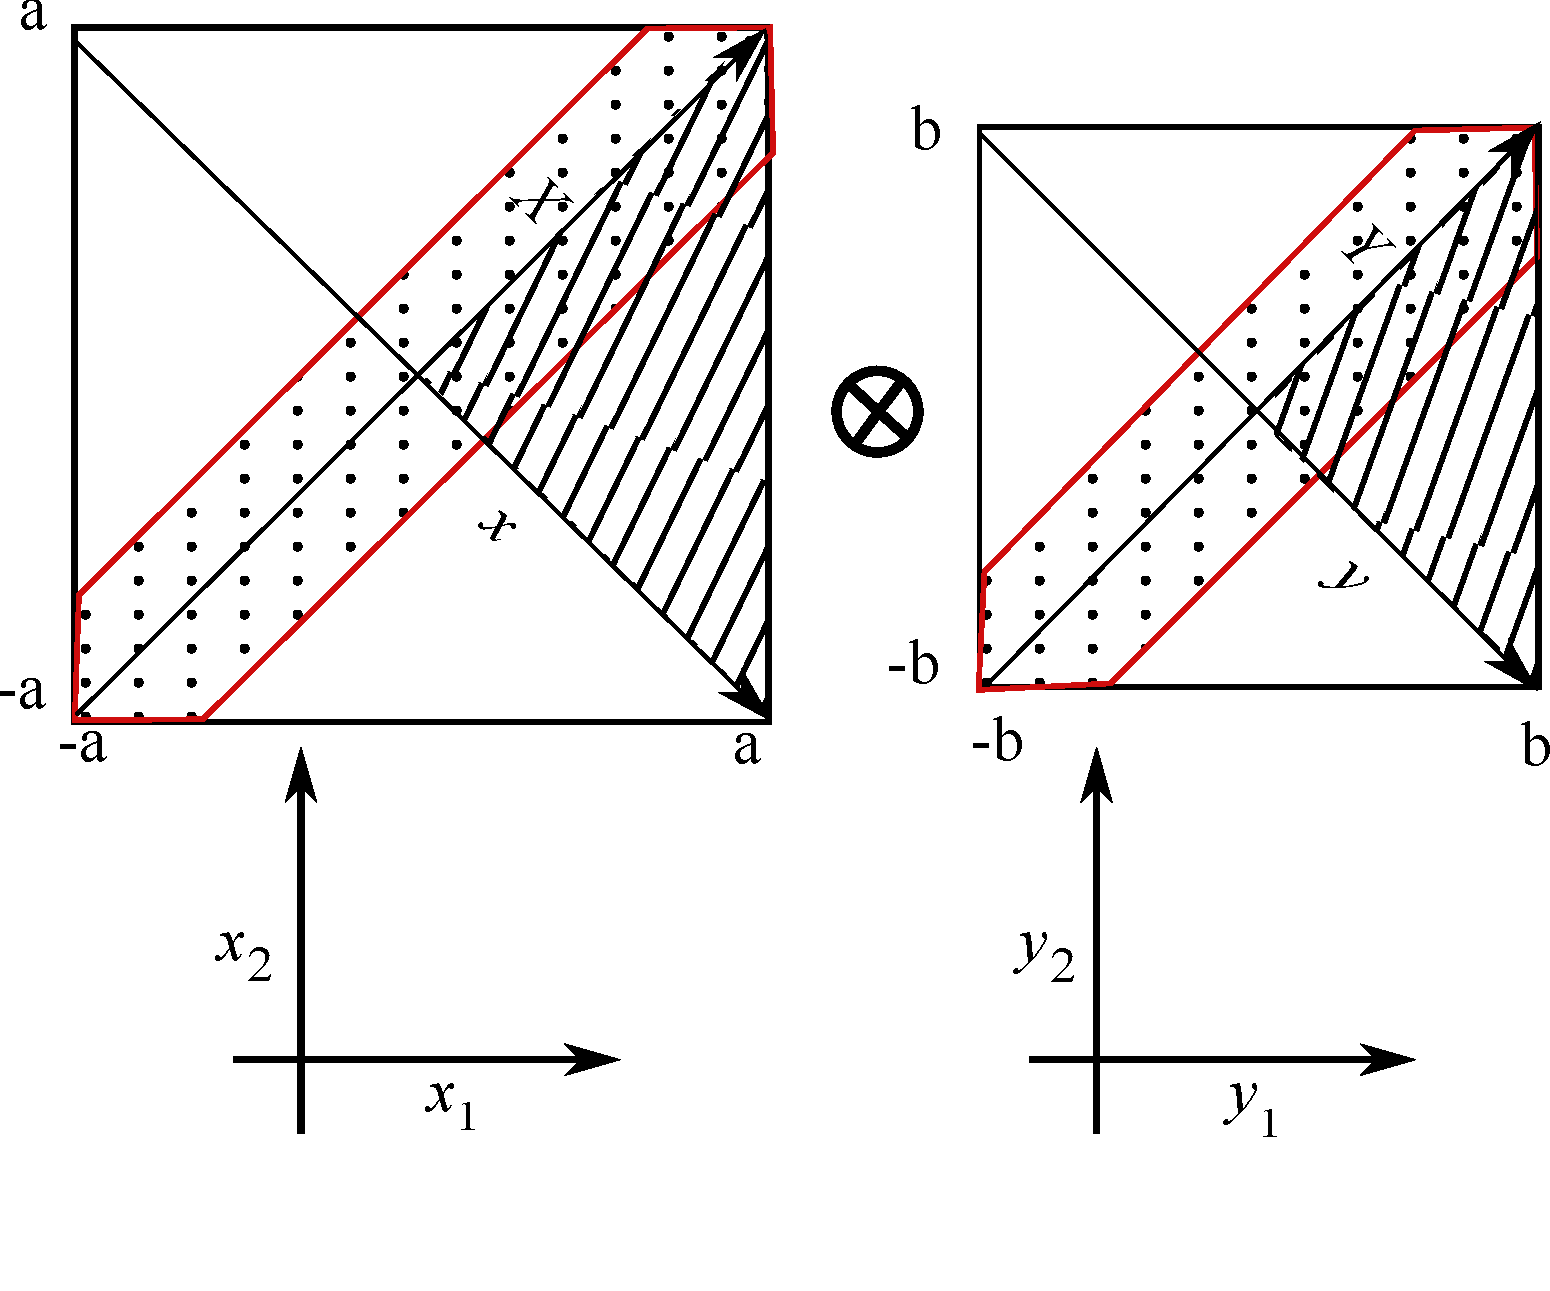
\includegraphics[width=0.45\textwidth]{figures/diagramintegra01.pdf}
  \end{center}
  \caption{The space to integrate is the product of the spaces
    corresponding to the horizontal and vertical coordinates. The dotted
    bands show the excluded set, that is, the complement of $Z$, where the condition 
    $ (x_1-x_2)^2 + (y_1-y_2)^2 \ge (2r)^2 $ is not satisfied.
    The width of each band is dependent on the particular 
    point of evaluation
    on the other subspace, which ranges from 0 to $r\sqrt{2}$. Due to symmetry, 
    we evaluate integral for X,Y,x,y>0 (indicated by hatches in the
    figure), and multiply by 16.
    \label{diagintegral01}  
    }
\end{figure}

It is easiest to represent the  
excluded cylinder in the coordinates defined in 
Eq.~\eqref{cambiocoor01}:

\begin{equation}\label{integraltotal}
  V_\text{free} = 
  \iint\limits_{\substack{ x=-a \sqrt{2} \\ y=-b \sqrt{2}}}
  ^{\substack{ x=a \sqrt{2} \\ y=b \sqrt{2}}}
   \mkern-9mu \rd x \rd y 
  \iint \limits_{\substack{X=-a\sqrt{2} + |x| \\ Y=-b \sqrt{2} + |y| }}^
  {\substack{X=a\sqrt{2} - |x| \\ Y=b \sqrt{2} - |y| }}
   \mkern-18mu  \rd X \rd Y
\, \indicator{ x^2 + y^2 \ge 2r^2  }.
\end{equation}

Since $X$ and $Y$ do not appear in the integrand, the corresponding integrals are trivial, giving
\begin{align}
  V_\text{free}  &=
  \iint\limits_{\substack{ x=-a \sqrt{2} \\ y=-b \sqrt{2}}}
  ^{\substack{ x=a \sqrt{2} \\ y=b \sqrt{2}}}
   \mkern-9mu \rd x \rd y 
2 \left( a \sqrt{2} - |x| \right) \, 2 \left( b \sqrt{2} - |y| \right) \indicator{ x^2 + y^2 \ge 2r^2 } \\
&=
16  \iint\limits_{\substack{ x= 0 \\ y=0 }}
  ^{\substack{ x=a \sqrt{2} \\ y=b \sqrt{2}}}
   \mkern-9mu \rd x \rd y  
\left( a \sqrt{2} - x \right) \left( b \sqrt{2} - y \right) \indicator{ x^2 + y^2 \ge 2r^2 },
\end{align}
where we have used the symmetry visible in Fig.~\ref{diagintegral01}.
Thus $V_\text{free} = 16(I_1 + I_2)$, where $I_1$ is the region where the range of
values of $y$
is affected by the exclusion condition, and $I_2$ is where the exclusion condition has
no effect on that range.
 In figure \ref{diagintegral01} this would correspond to the dotted and
white areas of the left diagram; see also Fig.~\ref{CasosIntegra} in the appendix. 
We have
\begin{align}
  I_1 &= \iint\limits_{\substack{x=0  \\ y = \sqrt{ 2r^2 - x^2}}}
    ^{\substack{x=r\sqrt{2}\\ y=b \sqrt{2}}} \! \rd x \rd y
\left( b \sqrt{2} - y \right)  \left( a \sqrt{2} - x \right) \\
&= 	
2 a b^{2} r  + \textstyle \frac{1}{6} (a+b) (2r)^{3} - \frac{1}{32}  (2r)^{4} - \frac{1}{4} {\left(\pi a b + b^{2}\right)} (2r)^2,
\end{align}
and
\begin{align}
  I_2 &= \iint\limits_{\substack{x=r\sqrt{2}  \\ y=0 }}
    ^{\substack{x=a\sqrt{2}\\ y=b \sqrt{2}}} \! \rd x \rd y
  \left( b \sqrt{2} - y \right)  \left( a \sqrt{2} - x \right)  \\
&=	
{\left( a^{2} - 2ar +   r^{2}\right)} b^{2}.
\end{align}
Thus 
\begin{align}\label{volumeabd}
 V_\text{free}
 & =  16 a^{2} b^{2}  - 16 \pi a b r^{2} + \textstyle \frac{64}{3} (a+b) r^{3}  - 8 r^{4} \\
&=: V_\text{prism} - V_\text{cyl},
\end{align}
as previously obtained by Munakata and Hu \cite{Munakata02}.
It is useful to split this expression into the total volume of the prism, 
$V_\text{prism}=16 a^2 b^2$, and the cylindrical volume excluded by the overlapping
condition, 
 $V_\text{cyl} =  16 \pi a b r^{2} - \textstyle \frac{64}{3} (a+b) r^{3}  + 8 r^{4}$.

The substitutions $a(r)\leftarrow (w-2r)/2$ and $b(r)\leftarrow (h-2r)/2$ give us
 the volume as a function of the radius, for fixed table size:
\begin{equation}\label{volumewhd}
 V_\text{free} 
= (w-2r)^{2} (h-2r)^{2}  - 
 \pi (w-2r)(h-2r) 4 r^{2} + 
\textstyle \frac{32}{3} (w+h-2r) r^{3}  
- 8^{4}.
\end{equation}

Note that the above formula is correct only when both
vertical and horizontal hopping are possible, i.e., when $h, w > 4r$.
If this is not the case, the 
integration limits for $X$ and $Y$ in \eqref{integraltotal} are altered, 
see Appendix~\ref{app:area_volume} for the corresponding results.

As an example, consider the case in which vertical hopping is possible
and horizontal is excluded, with $w \geq h$.
This case divides into two sub-cases: if
$ h \leq  w < 2 h $, there is a value of $r$ above which hopping is no longer possible,
but the discs still fit in the table. For $2 h \leq w $, vertical hopping is
possible until $ 2 r= h$ (where vertical movement becomes impossible). 
The configuration space splits into disjoint components, but 
thanks to the symmetry of
the problem, in some cases the cross-section areas and 
volumes become disjoint components sharing the same fraction of
the total volume, making the transition continuous. In other cases, we end with 
a discontinuity in the formulas,
corresponding to a factor of 2 or 4. 


For example, when $h/4 < r < w/4$ 
we define an auxiliary variable,
$c = \sqrt{4r^2-b^2}$. Then we have
\begin{multline}\label{VolumenCasoFeo}
V_{h/4<r<w/4} = 32abr^2 \left[ \arccos(b/2r)-\arccos(a/2r) \right]\\
+\frac{64 r^3}{3 } \left[ a((b-a)/2r)-b(c/2r+\sqrt{4r^2-a^2}/2r) \right]\\
+16 \left[ a b^2 c (4\sqrt{2}-1-\sqrt{2}/3) 
  +c^2b^2 (\sqrt{2}/3-1) \right]\\
-2r^2 (b^2-a^2)
\end{multline}

When $r$ is larger than both $h/4$ and $w/4$, one must take
into account a similar
contribution which inverts the roles of $a$ and $b$. Then there is
a case where hopping is impossible. 

%Omiti este parrafo ya que esta repetido abajo.
%For our numerical simulations, we take $w=1.5$, $h=1$, which avoids degenerate cases. 
%This covers all of the uses of the general volume formulas.
%Otherwise there is a case in which both hops become impossible simultaneously
%($h=w$), or cases in which one of them never gets excluded (e.g. $h>2w$).

We verified our expressions for the available space volume numerically using 
standard rejection-sampling Monte Carlo simulations, i.e. 
by generating uniform random positions for the disc centers in 
$[-a,a] \times [-b,b]$ and 
counting the fraction of initial conditions for 
which the two discs do not overlap (rejecting those where is overlap).
The results are shown in Fig.~\ref{VolMonteC}.
We chose the values $w=1.5, h=1$ for the numerical integration since all the different
cases of the volume formulas occur for these values: all hopps possible, only vertical
hopps possible, no hopps possible. This does not occur for all values of $w$, $h$,
for example if $h=w$ both hopps becomes impossible simultaneously and for $h>2w$
one of them never gets excluded.
%%%%% 

\begin{figure}[h]
\centering
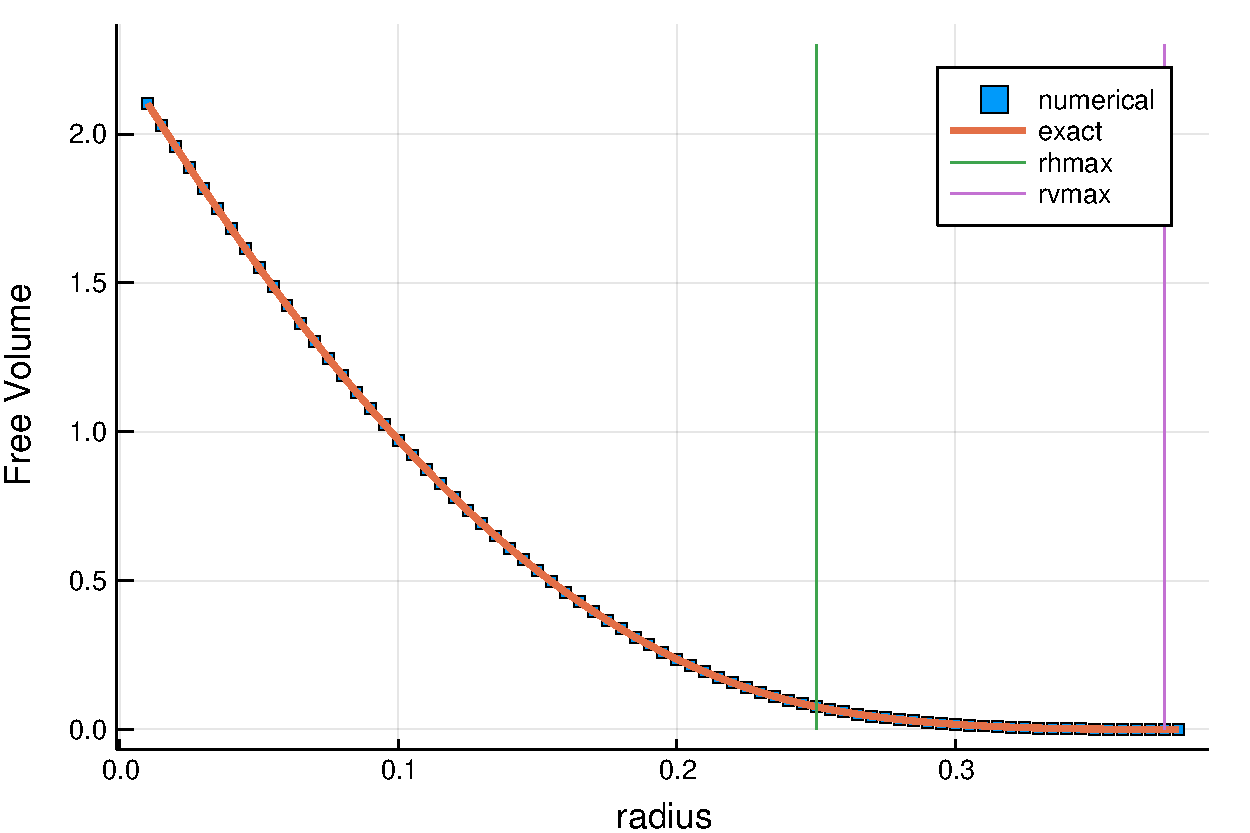
\includegraphics[width=0.45\textwidth]{./figures/FreeVolume01.pdf}
\caption{Free available volume in configuration space as function of radius. The
  line labeled $rhmax$ is the limit for horizontal hopping, and the one labeled
  $rvmax$ is the limit for vertical hopping. The transition between the formulas
is continuous.}
\label{VolMonteC}%% 
\end{figure}


The following subsections shall only show the formulas for $r<w/4, h/4$.
Bear in mind that some of the dynamics are possible above this limit,
it is only the position interchange that gets excluded. \\

%%
%% ¿Que ondas David, hacemos las simulaciones para el caso espantoso tambien?
%% Ok. Ya las voy haciendo


\subsection{Cross-section areas}\label{areahop}

The terms of the form $|A|$ in \eqref{meanfreetime} are surface areas of 3-dimensional surfaces (manifolds) $S$ embedded in the configuration space,
defined by algebraic equations of the form $g(\mathbf{x}) = 0$, so that $S = g^{-1}(0)$ is the zero set of $g$.
The surface area of $S$ is then given by
\begin{equation}
A(S) = \int \indicatorsymbol_Z(\mathbf{x}) \, \delta(g(\mathbf{x})) \, \mathrm{d} \mathbf{x}.
\label{eq:surface-area}
\end{equation}
To evaluate this, we use the following coarea formula
%relation in H\"ormanders Book, 
%sec 6.1 
\cite[section 6.1]{Hormander83} 
\begin{equation}
\int_{\mathbf{R}^d} f(\mathbf{x}) \, \delta(g(\mathbf{x})) \, \mathrm{d} \mathbf{x} = \int_{g^{-1}(0)}\frac{f(\mathbf{x})}{\| \mathbf{\nabla}g(\mathbf{x}) \|} \, \mathrm{d}S,
\label{eq:surface-dirac}
\end{equation}
where the integral on the right-hand side is over the surface $g^{-1}(0)$
\cite{Zappa2018}


The appearance of the normalization factor $\| \mathbf{\nabla}g(\mathbf{x}) \|$ can be understood intuitively by considering how to verify numerically these surface areas. One possible technique is to use rejection sampling to sample the volume given by $|g(\mathbf{x})| \le \eta$ for some small value of $\eta$. Points will be accepted or rejected according to their orthogonal distance to the surface, which is the factor in the denominator in the above expression. Our case is simple in this respect: most of our surfaces are either parallel to the coordinates or are in some way ``diagonal'', giving constant factors.
%$| \mathbf{\nabla}g(\mathbf{x}) \| )\sqrt{2}$ constant for all points. 
%%%% Removi esta linea porque se parece mucho a ""The main difficulty in the analysis is correctly accounting for several geometric factors with different origins in both the analytical and numerical calculations."
%The main difficulty in these calculations is correctly accounting for the factors arising in this way.

%Failing to take this constants into account produce some curious results: both analytical
%and numerical calculation of the areas can be wrong by the same factor,
%thus passing unnoticed until one tries Szabo's formula and end up being
%$\sqrt{2}$ times wrong.

%The efficiency could be improved by a Markov Chain Monte Carlo algorithm that rejects steps that take the dynamics outside the set of interest.

\subsubsection{Hopping}

Vertical hopping occus when the vertical positions of the two discs are equal: $y_1 - y_2=0$. In the language of the previous subsection, we take
 $g_\mathrm{hop}(x_1, x_2, y_1, y_2)= y_1 - y_2$, with gradient $\nabla g_\mathrm{hop}(\mathbf{x}) = (0, 0, 1, -1)$, so that $ \| \nabla g_\mathrm{hop}(\mathbf{x}) \| = \sqrt{2}$. 
 Alternatively, we can integrate 
directly in the $(x,X,y,Y)$ coordinates, where we use
$g(x,X,y,Y) = y$, and then return to the original coordinates. This results in the following expression:
\begin{widetext}
\begin{equation}
  A_\text{hop} =
\iiiint
\limits_{\substack{x_1, x_2 = -a \\ y_1, y_2 = -b}}^{\substack{x_1, x_2 = a \\ y_1, y_2 = b}}
\rd x_1 \rd x_2 \rd y_1 \rd y_2 
 \, \indicator{ (x_1-x_2)^2 + (y_1-y_2)^2 \ge (2r)^2 } \, \delta \big(\frac{y_1-y_2}{\sqrt{2}}\big).
\end{equation}
\end{widetext}
Carrying out the integrals  (see Appendix A) gives
 \begin{equation}\label{AreaH}
 A_\text{hop}  =  16 \sqrt{2} b(a-r)^2.
\end{equation}
As before, the formula is no longer valid for $r > w/4$. In this case,
vertical hopping becomes impossible for a larger radius.

Monte Carlo simulations to calculate this area must also
take into account the factor $\sqrt{2}$ (see Appendix B).
In this case we counted the proportion of successful placements of hard discs 
for which the distance 
$|y_1 - y_2|$ was within a small tolerance of $0$. 
Results are shown in figure \ref{AreaHopp01}.

\begin{figure}[h]
\centering
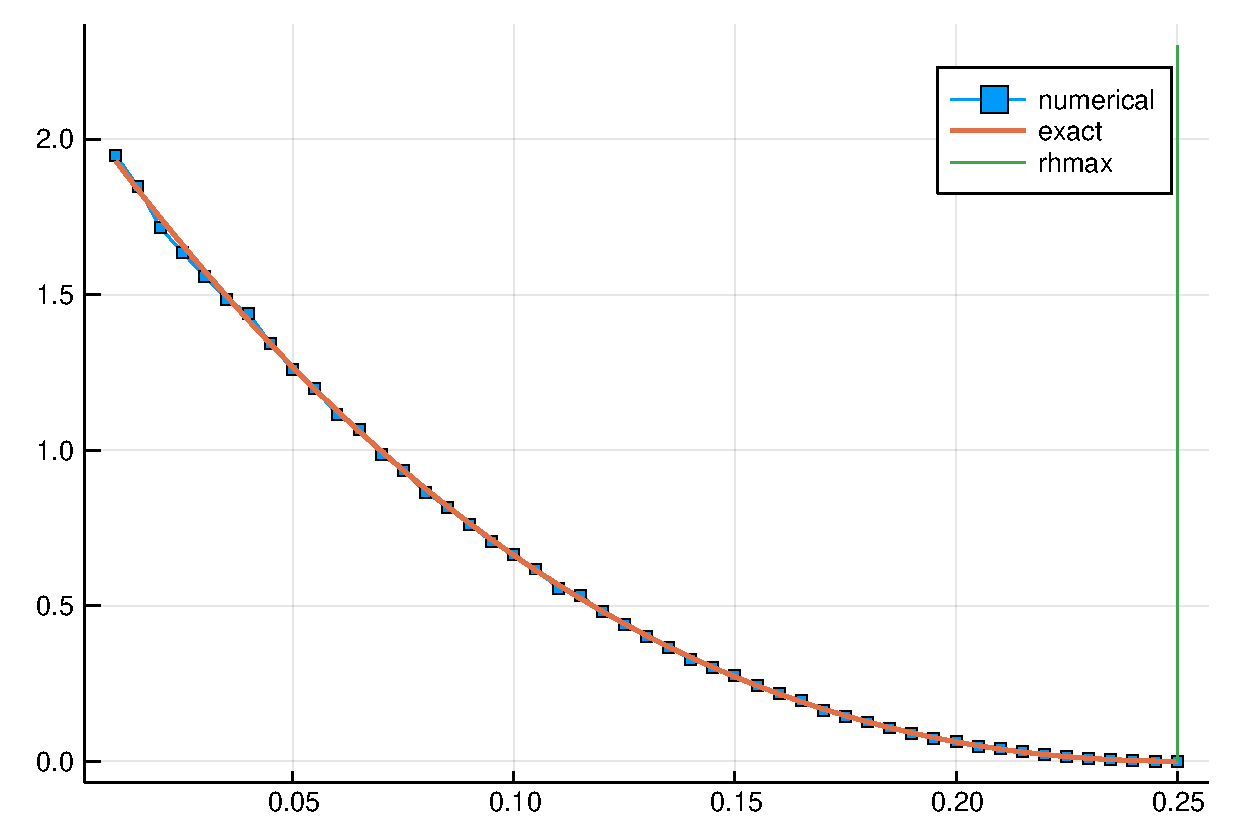
\includegraphics[width=0.45\textwidth]{./figures/AreaHop01.pdf}
\caption{The hopping area, $A_\text{hop}$, 
  indicated in the formula in eq. \ref{AreaH}. As explained in the text
in the text, the formula does not apply for $r>1/4$, but numerical values correctly
remain at zero.}
\label{AreaHopp01}
\end{figure}


\subsubsection{Disc collisions}

The area which represents collisions between the two discs is the surface area of the cylinder
that lies within the prism, given by
$$g_\text{coll}(\mathbf{x}) := (x_1 - x_2)^2 + (y_1 - y_2)^2 - 4r^2, $$
so that
$$\nabla g_\text{coll}(\mathbf{x}) = (2 (x_1 - x_2), -2(x_1 - x_2), 2(y_1 - y_2), -2(y_1 - y_2)),$$ 
with norm $\| \nabla g_\text{coll}(\mathbf{x}) \| = 2\sqrt{2} \sqrt{(x_1 - x_2)^2 + (y_1 - y_2)^2}$.

%The factors have the same reasons to appear as in the case of the hop condition.

For $r<w/4$, we find for the corresponding area
\begin{align}\label{AreaChoque}
A_\text{coll} & =  \sqrt{2} (
16\pi a b r -32 (a+b)r^2 +16 r^3).
\end{align}

We proceed in the same manner as last section, checking numerically which
random configurations
fall within a small tolerance from the collision condition, and
plotting this as a fraction of the total volume. The result is shown in Fig.~\ref{AreaChoqueTeoyNum}. 
\begin{figure}
\centering
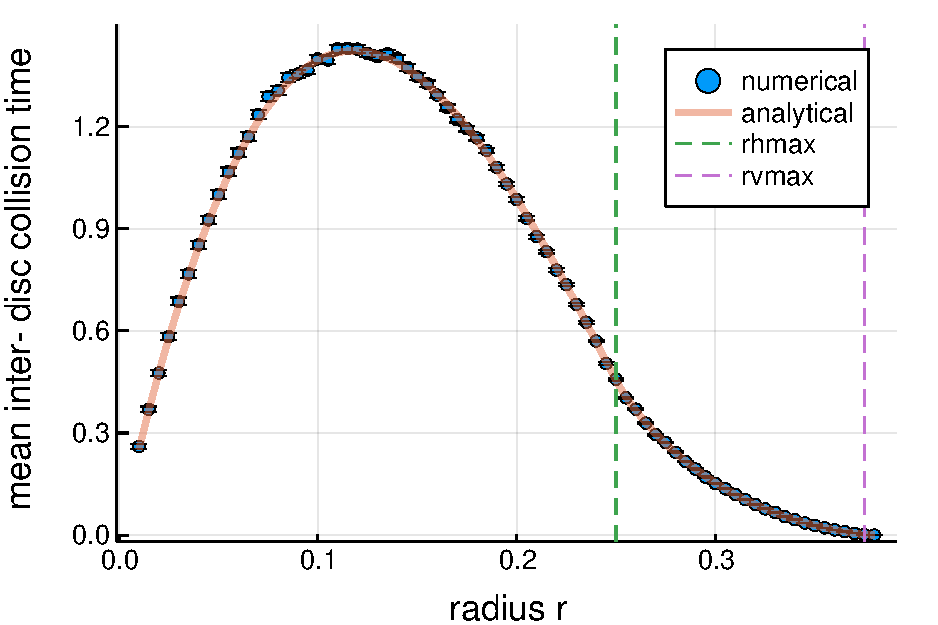
\includegraphics[width=0.45\textwidth]{./figures/AreaCol01.pdf}
\caption{Numerical and theoretical area 
for collision between the discs.  The theoretical formula 
\eqref{AreaChoque} breaks down at
$r > 1/4$, but we have here used the general formula \ref{app:colgeneral}
that appears in the Appendix.}
\label{AreaChoqueTeoyNum}.
\end{figure}


\subsubsection{Wall collisions}

We restrict attention to collisions of disc $1$ with the right wall, for which
$$g_\text{wall}(\mathbf{x}) := x_1 - a.$$
The corresponding area, after taking the delta function into account, is
\begin{equation}\label{areaindic}
  A_\mathrm{wall} =  \iiint \limits_ {\substack{x_2 = -a \\ y_1, y_2 = -b }}^
  {\substack{x_2=a\\ y_1,y_2=b}} 
   \rd x_2   \rd y_1   \rd y_2 \, \indicator{ (a-x_2)^2 + (y_1-y_2)^2 \ge 4 r^2 }
\end{equation}
The integration gives
\begin{align}\label{areax1p}
 A_\mathrm{wall} & = 8 a b^2-4  \pi b r^2 +\frac{16}{3}r^3 .
 % & = 2(w-d)^2 (h-2)^2- \frac{\pi}{2} (h-d) d^2 +\frac{2}{3}d^3 
\end{align}
Once again, a simple Monte Carlo procedure verifies this result,
shown in Fig.~\ref{area1derecha}. 
This time, the correction factors of $\sqrt{2}$ do not appear, since
the areas are orthogonal or parallel to the original
position coordinates.


\begin{figure}
\centering
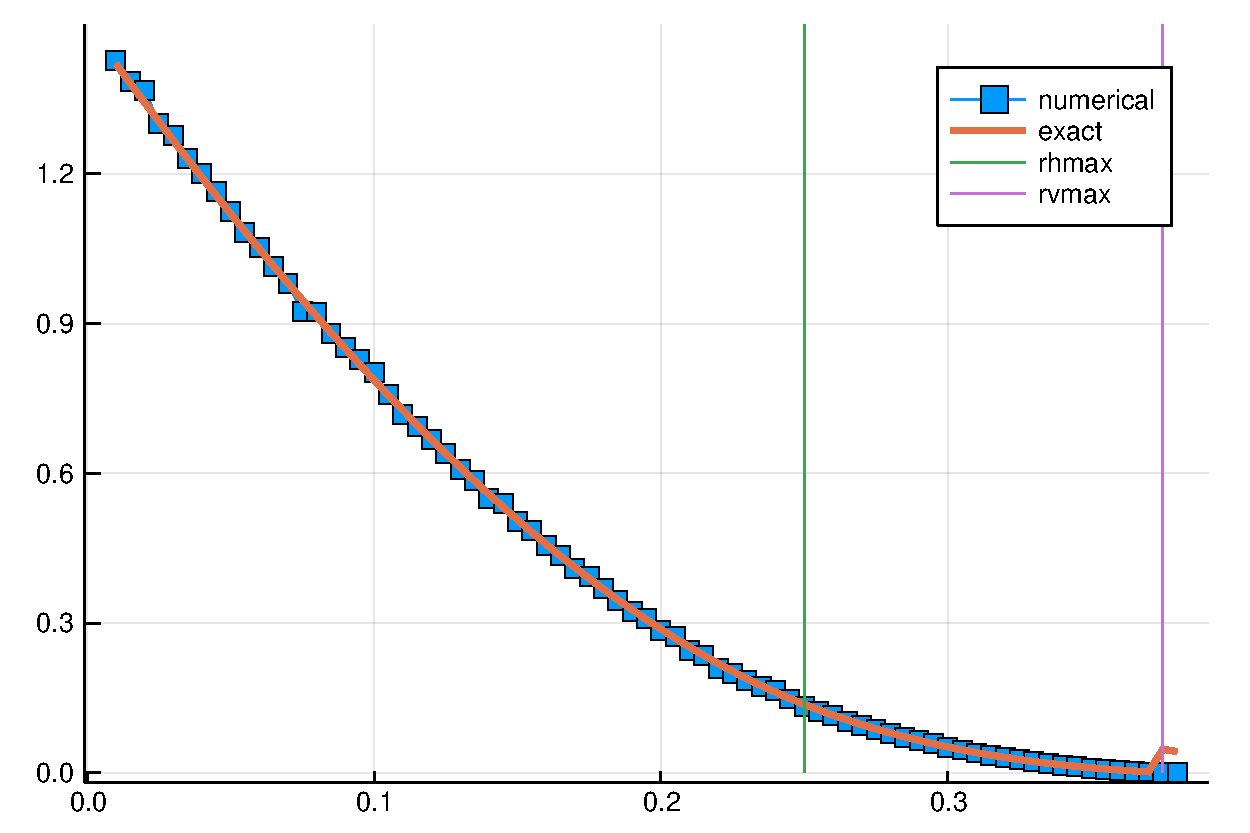
\includegraphics[width=0.45\textwidth]{./figures/AreaWall01.pdf}
\caption{Numerical and theoretical calculation for the area
for the impact of a particular disk with the right wall, as in \eqref{areaindic}.
Again, the general formula has been used.}
\label{area1derecha}.
\end{figure}

Taking into account the symmetry of the expression for either disc
 bouncing on either of the vertical walls, the
area for this event is  $4A_\text{wall}$. For horizontal wall 
collisions, the roles of $a$ and $b$ are switched.
Thus the area for any impact on any wall is
\begin{align}\label{areawalls}
 A_\text{walls} & = 32 a b (a+b)-16 \pi r^2 (a+b) +\frac{128}{3}r^3.
 %&=  4 (w-d) (h-d)  (w+h-2d) -2 \pi d^2 (w + h-2 d) +\frac{16}{3}d^3. 
\end{align}
%The cross section area for any collision is then 
%the sum of the last expression
%and the area for collisions between discs, \eqref{AreaChoque}.


\section{Exact mean event times}

In this section, we apply the results of the last section to give
exact mean inter-hop times, as well as wall collision and disc collision times.
The analytical results have been tested against numerical simulations.
The latter where obtained via Monte Carlo initial conditions and standard
billiard dynamic simulations. The trayectories of the centers of the
discs are determined by their momentum and the first collision
(either with wall or between discs) is given by
the one that produces a smaller positive time. The discs are then set into its new
position at the event, new momenta are calculated.
and the procedure is repeated. 
%%%%%%%%%% Why is the first event time discarded???
The first event time is discarded. Hopping
times can be inferred by retracing the collisions and filtering those that have
changed the sign of the difference of the coordinates in question (either
horizontal or vertical). The exact time can be determined from
the momenta between the beforehand collision and the afterwards one.
In order to
obtain more reliable statistics, specialized subroutines where written
such that only one kind of event was tracked. %%%%%%%%%%%%%% Aca tampoco entiendo porque medir cada evento por separado hace las estadisticas mas confiable
All the code is avaible as a Jupyter/Julia Notebook. %%%%% anadir link/referencia 


\subsection{Mean hopping time}

 
Inserting the results of the previous section 
into the formula for the mean times for crossing
surfaces of section \eqref{meanfreetime}, finally gives exact mean inter-event times.

For vertical
hops we have
\begin{equation}\label{hoptau}
 \mean{\tau_\text{hop}} = 	
\frac{3 \pi}{4\sqrt{2}}
\frac{2 a^{2} b^{2}  - 2 \pi a b r^{2} + \textstyle \frac{a+b}{3}  (2r)^{3}  -  r^4}
{ b \sqrt{2}  ( a - r )^2}.
\end{equation}
Recall that here there is a factor $s = 2$.

In the limit of small disc radius, the discs have almost no interactions, and the result depends only
on the table height:
\begin{equation}\label{hoptaulimit}
 \mean{\tau_\text{hop}} \overset{r \to 0}{\sim}
\frac{3 \pi}{8\sqrt{2}}h.
\end{equation}

Also of interest is the limit $r\sim w/4$, where vertical hopping becomes
impossible.  The lower term goes to zero quadratically, while the available volume
is still positive (except in the degenerate case $w=2h$). The exact expression
is cumbersome, due to the fact that the general volume expression contains trigonometric functions
 and is unintuitive (see Section~\ref{app:volume}),
but the leading term in the numerator is  $w^2(h/2-w/4)^2$, and the denominator
stays the same, so
it goes to infinity
like $1/x^2$. The figure \label{MeanHopp01} shows the comparison between
numeric and analytic results for the complete valid range. Notice the abrupt
change in behavior as we approach $r_{vmax}$.


\begin{figure}[h]
  \centering
  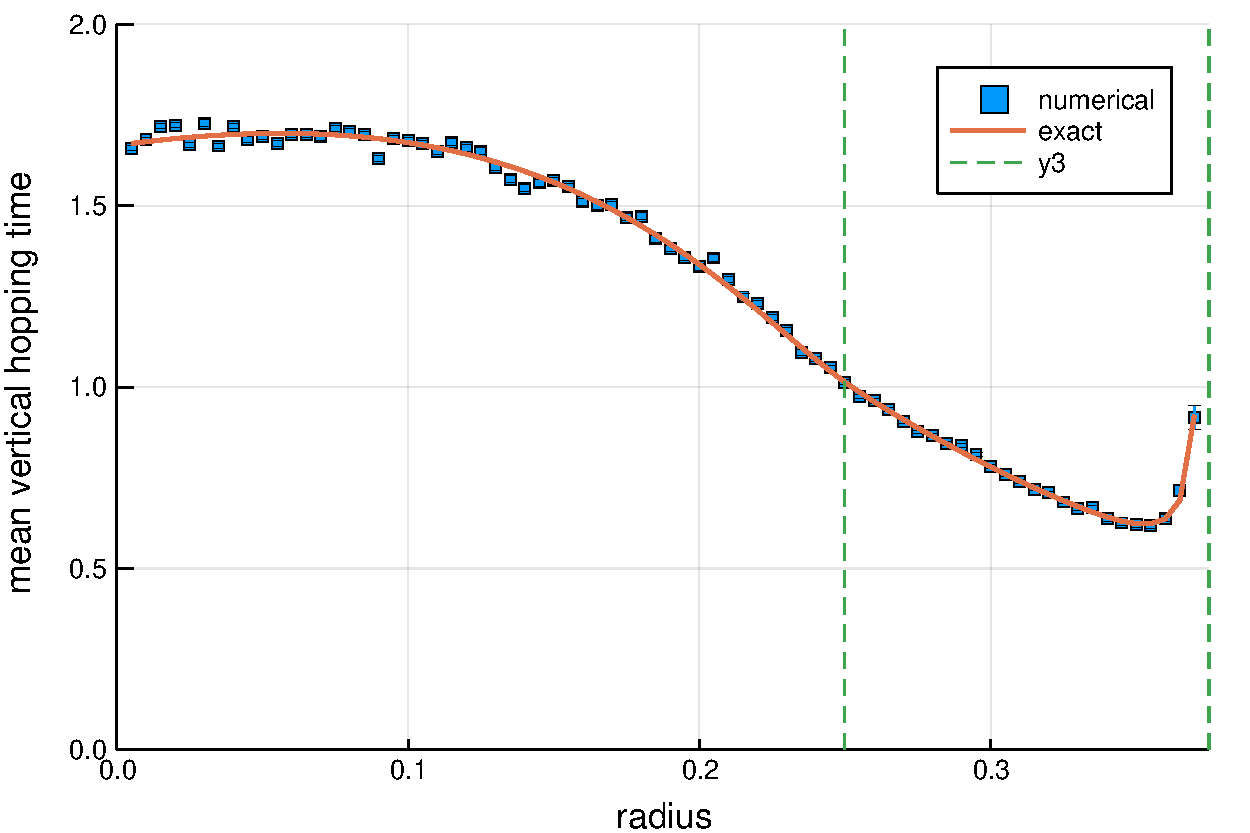
\includegraphics[width=0.45\textwidth]{./figures/VertHop01.pdf}
  \caption{Mean hopping time as function of the radius.}\label{MeanHopp01}
\end{figure}


\subsection{Mean disc collision time}

For collisions between discs, we have, for the case $r < w/4$,
\begin{equation}\label{colltau}
 \mean{\tau_\text{coll}} = 	
\frac{3 \pi}{2\sqrt{2}}
\frac {2 a^{2} b^{2}  - 2 \pi a b r^{2} + \textstyle \frac{a+b}{3}  (2r)^{3}  -  r^4}
{2\pi a b r -4(a+b)r^2+2r^3}.
\end{equation}
As expected, this tends to infinity in the limit of small radius, with asymptotics
\begin{equation}\label{colltaulim0}
\mean{\tau_\text{coll}} \overset{r \to 0}{\sim}
\frac{3}{8\sqrt{2}}\frac{wh}{r}.
\end{equation}

For the case in which the discs narrowly fit inside the table we need to
use the more cumbersome expression in \eqref{VolumenCasoFeo} and
the corresponding area. The time between collisions should go to zero; 
see figure~\ref{MeanCol01}. In this case, the function is smooth for the whole
range of valid values for $r$.

\begin{figure}[h]
  \centering
  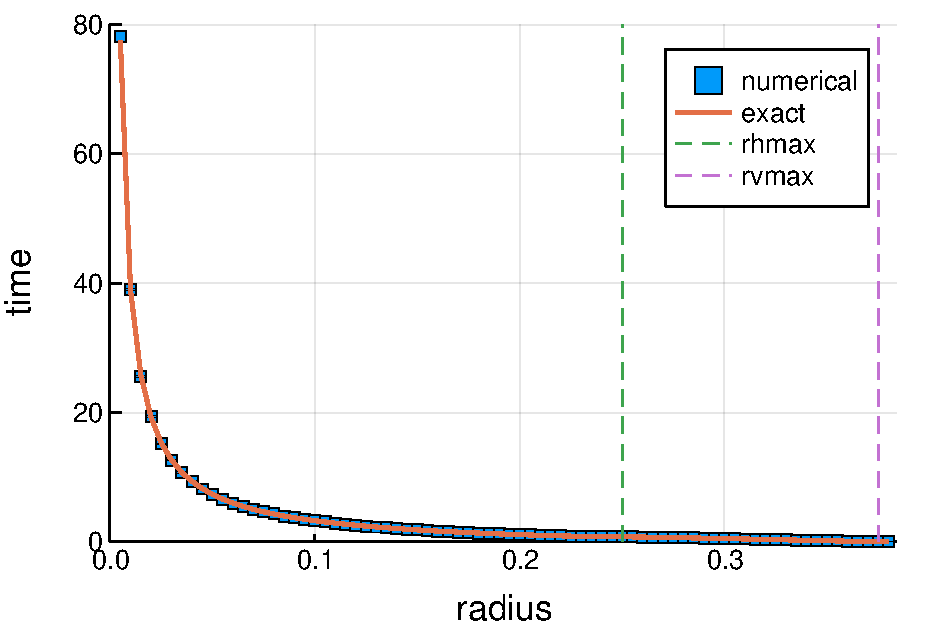
\includegraphics[width=0.45\textwidth]{figures/DiscCollisions01.pdf}
  \caption{Mean disc collision time as function of the radius. }\label{MeanCol01}
\end{figure}



\subsection{Mean wall collision time}

Lastly, for a specific disc colliding with a specific vertical wall we have
\begin{equation}\label{impactwall}
 \mean{\tau_\text{wall}} = 	
\frac{3 \pi}{2\sqrt{2}}
\frac { 2a^{2} b^{2}  -  2\pi a b r^{2} + \frac{a+b}{3}(2r)^3 - r^4}
{ab^2-\pi/2b r^2 + \frac{16}{3} r^3 },
\end{equation}
in the case that $r<h/4$. The limiting form for small $r$ depends
only on the width of the table and is exactly
$3\pi w/2$. In the numerics this appears as the intersection with the $\tau$
axis. %%%%%%%????????????

For the case that $r\approx h/4$ we would have two limiting forms,
as there is a discontinuity in the available Volume, but it is exactly
a factor of two. In the comparison with numerics, we can see
this jump in the function, accompanied by a larger error in the
calculations (since it is harder to find correct starting positions). 
This is indicative of 
the system breaking into smaller ergodic components.


\begin{figure}[h]
  \centering
  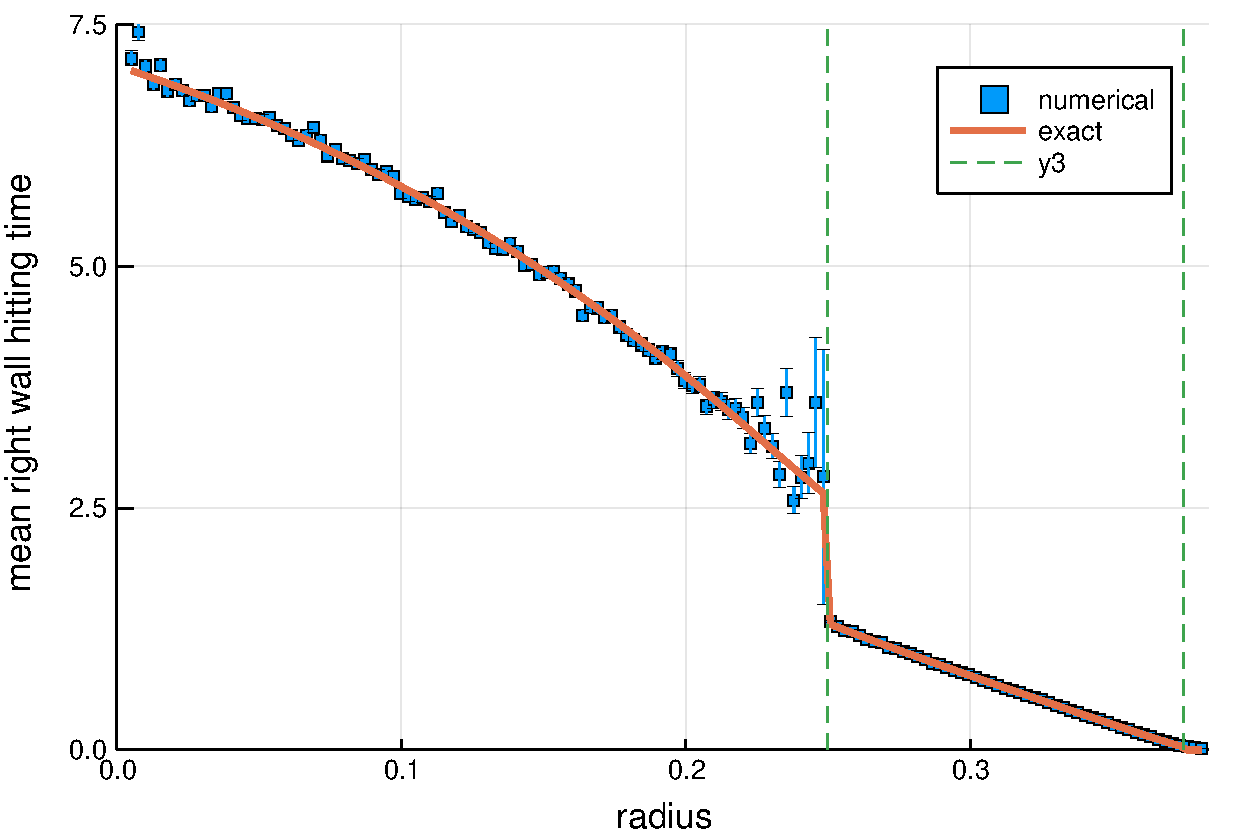
\includegraphics[width=0.45\textwidth]{./figures/HitRightWall01.pdf}
  \caption{The mean impact-on-walls time as function of the radius, 
  %Again, same
    notes as the figure \ref{MeanHopp01}}
    \label{MeanImp01}.
\end{figure}



%
\section{Distributions}

Since each type of event time that we study is a recurrence time to a
certain surface in phase space, we expect to observe the standard
exponential distribution for return times of hard chaotic systems
\cite{Hirata1999}. It is known that deviations from the
exponential depend on the particularities of the system at hand
\cite{Altmann2005}.

%In this system the relevant phase space on the
%energy surface is seven dimensional. That means that
%KAM islands if they exist are irrelevant (of measure zero)
%and the system is an example of hard chaos. Such systems
%have this exponential behaviour in their recurrence times. 

As an example, we explore
the distribution of hopping times for different radii and find that the
distribution depends both qualitatively and quantitatively on the
radius, with the expected exponential decay being observed in the middle section
of the distribution. 


\begin{figure}[h]
  \centering
  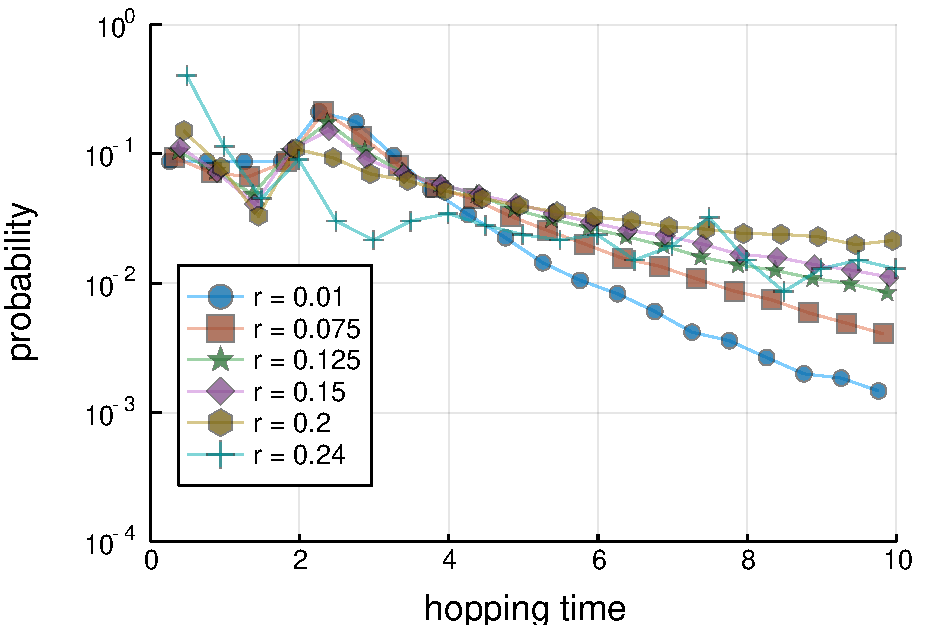
\includegraphics[width=0.45\textwidth]{figures/histogram_hopping_times.pdf}
  \caption{Histogram of hopping times.}
    \label{histogram_hopping}.
\end{figure}


\section{Conclusions}

We have calculated exact analytic expressions for mean hopping and
collision times in the paradigmatic model of two discs in a hard box,
by treating them as return times to appropriately-chosen surfaces of section, %%%%% surfaces of section?
and applying results from ergodic theory.
%using 
%extensive theory of chaotic billiards. The subjacent theory
%of ergodic systems already contains strong theorems and formulas
%that only need judicious  application to show their 
%predictive power. 
%The step done by Machta and Zwanzig in
%that direction is an example of bringing to the ground those
%ideas to applicable problems. 
%We have expanded
%that line by showing a large class of events can be modeled
%as return times to appropriately chosen surfaces of section. 
The analytical results derived 
confirm the limiting behavior obtained
by Bowles \etal \cite{Bowles04} by a different method, and are in excellent agreement with Monte Carlo simulations.

The results may be extended to discs with different radii, considering two parameters,
$r_1$ and $r_2$. That would give some bifurcations in cases, that could
produce scenarios in which hopping is always permitted or that one of the
discs cannot be larger (or cannot move anymore,
blocking sections of the configurations space), but the other still has space to use. 
The integrals would be similar as those presented here, but the space avaible
would change.  
On the other hand more spatial dimensions could increase not
only the algebraic difficulty, but the grasping of the posible scenarios.
Even with spheres bouncing inside a three dimensional box,
hopping can occur in multiple not intuitive ways. As an example,
there may be not enough space to interchange $x$ position
\emph{in the same plane}, but there may be a way around that
is barely visible without an adecuate experiment or
simulation.%%%%%%%%%% dificil de entender


It would also be possible to extend the results to calculate exact mean collision
and hopping times for systems containing more discs,
but the analytical calculations become more challenging \cite{three_hard_discs_2004}.
In the limit of a large number of hard spheres, Chernov \cite{Chernov97}
was able to apply these methods to derive the exact limiting free flight time for a gas of hard spheres. Limiting case tend to overlock the scenario bifurcations that
can occur on specific instances. Hopping, in particular, would become very
messy after the addition of a third disc. Discs can block each other for long periods,
but not make a definitive block, and so on.

The work presented here deals with the simplest case for the problem at hand, but provides 
quantitative insight in the distribution of times and their
general behaviour. Furthermore, the results shown here could be applied for the design of a
random switch--with a known distribution of times. A microscopic table with two
fullerene balls may produce a similar dynamical system, and the change of positions
or the hit against walls be measured and used to trigger certain switches. 
Knowing the mean times and approximate distributions can be then used
to obtain the desirable switching times of a random, deterministic machine.

The known laws of behaviour of chaotic systems are powerful universal insights
into seemingly random motion. Nevertheless, each systems has its own
particularities which make it stand from the rest. The slight deviation from
these universal laws are a fingerprint of the underlying systems. By
accumulation of examples, we may gain insight into other problems that
present already seen behaviour. We hope that the distributions presented here
help in that direction. 

%We may simulate even more complex systems that could represent subtle interactions,
%such as that each disc is ``transparent'' to some wall and not another. Those
%modifications would simply change the avaible volume formulas, but would be
%tractable in a more or less straightforward manner. A posible setup would be to
%make every disk stay in a separate but overlapping box, representing some kind
%of territorial interaction ( this has been done with difussive motion).



%2 hard spheres in a spherical pore: conservation laws

\appendix
\section{General area and volume calculations}
\label{app:area_volume}

In this section, we find expressions for areas and volumes in all 
regimes.
%We use the same notation as in the rest of the paper.
To simplify the formulas, we omit the dependence
of $a$ and $b$ on $r$.



\subsection{Volume}\label{app:volume}


An implicit assumption was made on the limits of integration
in \eqref{integraltotal}. If $w, h > 4r$, then the limits of integration
are unaffected by the radius of the circles.
In order to avoid the same positive term $16a^2b^2$,  %%%%%%%suena m
in the formulas, we work here with
the excluded volume $V_\text{cyl}$, instead of the available one $V_\text{free}$. 


We begin the derivation after integrating out $X$ and $Y$:
\begin{equation}\label{VolumenGeneral}
\frac{V_{cyl}}{16}  =\iint \rd x \rd y \left[ 2ab-\sqrt{2}(ay+bx)+x y \right]
\indicator{x^2+y^2 < 2r^2 }.
\end{equation}
A diagram helps us visualize the limits of integration. The most general
case is (without loss of generality) $h < w < 2h$; as the disc radius 
%$r$ increases, we  pass through the following three regimes: from the regime where both vertical and horizontal
%hopping occur, to one in which only vertical hopping
%is possible, and then to  one in which no hopping is possible but movement
%can still occur. The three regimes are characterized by the following inequalities:
\begin{itemize}
\item Horizontal and vertical hopping possible: $0 <r \leq h/4$;
\item Only vertical hopping possible: $h/4 < r \leq w/4$;
\item No hopping possible: $w/4 < r < (h+w - \sqrt{2hw}) / 2$.
\end{itemize}
The largest possible radius is illustrated in Fig.~\ref{radiomaximo}.

\begin{figure}[h]
  \centering
  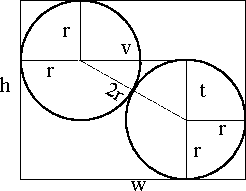
\includegraphics[width=0.4\textwidth]{figures/DiagramaRadioMaximo.pdf}
  \caption{The largest possible radius for $h<w<2h$. The auxiliary variable
    $v$ is the horizontal difference in coordinates between the centers,
    and $t$ the corresponding vertical one.
    From the diagram
    one can see that $t^2+v^2=(2r)^2$, $h=t+2r$ and $w=v+2r$, from which
    one can deduce the value for $r$.}
  \label{radiomaximo}
\end{figure}

We examine these regimes on the integration space. The first one is solved
in the main text, but we repeat it here using a different coordinate system
that proves useful. In Fig.~\ref{diaglimites} we present the three regimes as
the shaded area where we perform the integration. 
  
\begin{figure*}[h]
        \centering
        \begin{subfigure}[b]{0.32\textwidth}
          \centering
          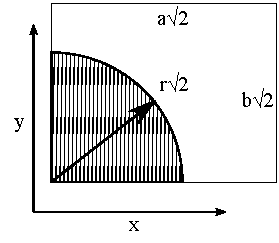
\includegraphics[width=\textwidth]{figures/DiagramaIntegraCaso1.pdf}
          \caption{$2r<h/2$}
          \label{Caso1}
        \end{subfigure}%
        ~ %add desired spacing between images, e. g. ~, \quad, \qquad etc.
        % (or a blank line to force the subfigure onto a new line)
        \begin{subfigure}[b]{0.32\textwidth}
          \centering
          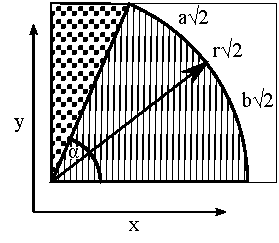
\includegraphics[width=\textwidth]{figures/DiagramaIntegraCaso2.pdf}
          \caption{$h/2<2r<w/2$}
          \label{Caso2}
        \end{subfigure}%
        ~ %add desired spacing between images, e. g. ~, \quad, \qquad etc.
          %(or a blank line to force the subfigure onto a new line)
        \begin{subfigure}[b]{0.32\textwidth}
          \centering
          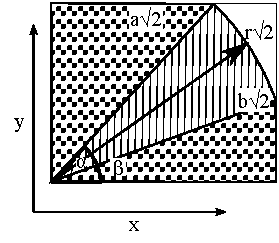
\includegraphics[width=\textwidth]{figures/DiagramaIntegraCaso3.pdf}
          \caption{$w/2,h/2<2r$}
          \label{Caso3}
        \end{subfigure}%
        \caption{Three hopping regimes.
          The integral must be evaluated over the shaded region.
          It is divided in two cases: 
           the hatched area is
          solved by polar coordinates as in eq. \ref{app:volcyl},
          and the dotted area indicates the part of the integral
          that is carried away in Cartesian Coordinates as in eq.
          \ref{app:voldot}.
          In the first case all hopping is possible; the middle case
          allows only for vertical hopping; and the last case excludes hopping.}
\label{CasosIntegra}
\end{figure*}
The shaded area in Fig.~\ref{CasosIntegra} represents the region in which the indicator function
has value 1. 

We evaluate the integral--carefully choosing the limits of integration. We perform the integral over the hatched area in polar coordinates $(\rho, \theta)$.
We call the integral $V_h(r,\alpha,\beta)$ (where $h$ stands for ``hatched''). %%% Removi la palabra "indefinite" ya que el termino indefinite integral no es apropiado aqui puesto que la integral tiene limite superior e inferior.
As can be seen from figure \ref{CasosIntegra}, the all hopping possible regime
corresponds to $\alpha = \pi/2, \beta=0$, the vertical hopping regime is where
$\alpha < \pi/2, \beta=0$, and the no-hopping regime is where $0 < \beta< \alpha < \pi/2$.

We rewrite the integral in terms of an angle $\theta$:

\begin{equation}\label{app:volcyl}
\begin{split}
\frac{V_h(r,\alpha,\beta)}{16} &=
\iint \rd x \rd y \left[ 2ab-\sqrt{2}(ay+bx)+x y \right]
\indicator{x^2 + y^2 < 2r^2}\\
&=
\iint \rd \rho \rd \theta \rho 
\left[ 2ab -\sqrt{2}(a\rho\sin\theta+b\rho\cos\theta) \right. \\
& \qquad + \left. \rho^2 \cos\theta\sin\theta \right]
\indicator{\rho^2<2r^2 }
\end{split}
\end{equation}
The indicator function determines the limits for the $\rho$ integration variable.
We set $\alpha, \beta$ as the other two limits and perform the
integral over $\rho$, which does not change in the three regimes.
\begin{widetext}
\begin{equation}
  \begin{split}
    \frac{V_h(r,\alpha,\beta)}{16} &=
    \iint\limits_{\beta,0}^{\alpha,r\sqrt{2}} \rd \rho \rd \theta \rho
    \left( 2ab -\sqrt{2}(a\rho\sin\theta+b\rho\cos\theta) 
    +\rho^2 \cos\theta\sin\theta \right)\\
 &=\int\limits_\beta^{\alpha}  \rd \theta  
\left[ 2abr^2 - r^3 4/3 (a\sin\theta+b\cos\theta)+r^4 (\cos\theta\sin\theta) \right].\\
\end{split}
\end{equation}
\end{widetext}
Now we integrate over the $\theta$ variable:
\begin{equation}\label{Volrtheta}
  \frac{V_h(r,\alpha,\beta)}{16} = 2r^2ab\theta
  +4/3r^3(a\cos\theta-b\sin\theta)
  +\frac{r^4 \sin^2\theta}{2} \Bigg\vert_\beta^\alpha.
\end{equation}
For the case in which all hopping is posible, the expression in \eqref{Volrtheta}
takes the values $\alpha=\pi/2, \beta=0$ and after multiplying by 16 both sides,
we recover the Munakata and Hu formula. For the other two cases, we use that
$\sin \alpha = b / r$ and $\cos \beta = a / r$.




Now we treat the dotted areas in the figures \ref{Caso2} and \ref{Caso3}. Since they are triangular, they
are more easily treated in Cartesian coordinates. We start with the upper
triangular region
and show the procedure, and then we cite the result for the
other triangle.
First, we realize that as we are inside the triangle, the characteristic function
translates to a simple integration limit:

\begin{widetext}
\begin{equation} \label{app:voldot}
  \begin{split}
    V_{u}(r) /16 &=\iint \rd y \rd x [2ab-\sqrt{2}(ay+bx)+xy] \indicator{(x)^2+(y)^2<2r^2 }\\
    &=\int_0^{b\sqrt{2}}\rd y \int_{0}^{y\sqrt{r^2-b^2}/b} \rd x [2ab-\sqrt{2}(ay+bx)+xy] \\
   &=\int_0^{b\sqrt{2}}\rd y \bigl[2abx-\sqrt{2}(ayx+bx^2/2)+x^2y/2\bigr]_{0}^{y\sqrt{r^2-b^2}/b} \\
      &=\int_0^{b\sqrt{2}}\rd y
        \bigr[
          2aby\frac{\sqrt{r^2-b^2}}{b}
          -\sqrt{2}
          \bigr(
          \frac{ay^2\sqrt{r^2-b^2}}{b}
            +\frac{y^2(r^2-b^2)}{2b}
            \bigl)
           +\frac{y^3(r^2-b^2)}{2b^2}
           \bigl]\\
        &= \Bigr[ay^2\sqrt{r^2-b^2}-
          \frac{\sqrt{2}y^3}{3}
          \bigr(
          \frac{r^2-b^2+2a\sqrt{r^2-b^2}}{2b}
            \bigl)
            +\frac{y^4(r^2-b^2)}{8b^2}
            \Bigl]_0^{b\sqrt{2}}\\
          &=2ab^2\sqrt{r^2-b^2}
          -\frac{2b^2(r^2-b^2+2a\sqrt{r^2-b^2}}{3}+\frac{b^2(r^2-b^2)}{2}\\
          V_{u}(r)&=32ab^2\sqrt{r^2-b^2} -\frac{32
            b^2}{3}(r^2-b^2+2a\sqrt{r^2-b^2}) +8b^2(r^2-b^2).
  \end{split}
  \end{equation}
The procedure is similar for the lower dotted  region in Fig.~\ref{Caso3},
and gives a symmetric expression:
\begin{equation}
          V_{l}(r)=32a^2b\sqrt{r^2-a^2} -\frac{32
            a^2}{3}(r^2-a^2+2b\sqrt{r^2-a^2}) +8a^2(r^2-a^2).
\end{equation}
\end{widetext}

These expressions account for all volume available in the configuration space, but
cannot be used for calculation of all event times that interest us. We need also
expressions that take into account that this space is divided into disjoint components,
as some events become impossible in each of these subsystems. For example,
(see the next section), disc 1 cannot hit the left wall if
it started on the right and horizontal hopping is excluded. So we have to
take into account that only half of the positions are available (due to symmetry)
 in \eqref{meanfreetime}.

Due to the symmetry of the problem, the available volume
for each disjoint component of the dynamical system is equal; for example, if horizontal hopping is no longer possible
($w/4<r<h/4$), then there are two symmetric disjoint components: the system
starting with disc 1 on the left and the one starting with disc 1 on
the right. Both occupy the same phase space volume, as they are
symmetric under interchange of labels. If $h<4\leq r$ then the system gets further
divided into four disjoint components. 



\subsection{Area}

The above procedure must be repeated for the different
area calculations. We use a suitable Diracdelta to represent each codimension-1 collision
event (touching of a disc with a wall or another disc). We multiply the characteristic function of the available space by the Dirac delta, and
then again divide it into the three cases, namely, all hopping, only vertical hopping
and no hopping possible, again referring to Fig.~\ref{CasosIntegra}.
Sometimes it turns out to be easier to obtain 
the integral  over all configuration space and then exclude the part that
corresponds to the overlapping condition. Again, the hatched area of the exclusion
condition has a simpler representation in polar coordinates, and the triangular
(dotted) regions can be treated in rectangular coordinates.
%
%The areas representing different types of collision events require careful treatment of Dirac delta operators.
%In general, an event is represented by a certain constraint of the form
%$f(x_1, x_2 , y_1,y_2) =0 $; the measure of the corresponding three-dimensional manifold (surface) in configuration space is, in general,
%\begin{equation}
%  A_f=\iiiint \rd {x_1}  \rd {x_2}  \rd {y_1}  \rd {y_2}
%  \frac{\delta(g(x_1, x_2 , y_1,y_2))}
%  {\lVert \nabla f \rVert}
%  \indicator{(x_1-x_2)^2+(y_1-y_2)^2>4r^2 }.
%\end{equation}
%The factor $1/ {\| \nabla g \|}$ appears due to the fact
%that the measuring process must be done orthogonormally to the surface. 

\subsubsection{Hopping cross section}

The hopping cross section is a good example; see Fig.~\ref{DiagramaDelta01}. %%%%%%% a good example of what??
This is given by $g_\text{hop}(\mathbf{x}) = y_1 - y_2 = 0$:

\begin{widetext}\label{ahopcart}
\begin{equation}
  A_\text{hop} =
\iiiint
\limits_{\substack{x_1, x_2 = -a \\ y_1, y_2 = -b}}^{\substack{x_1, x_2 = a \\ y_1, y_2 = b}}
\rd x_1 \rd x_2 \rd y_1 \rd y_2 
 \, \indicator{ (x_1-x_2)^2 + (y_1-y_2)^2 \ge (2r)^2 } \, \delta \big(\frac{y_1-y_2}{\sqrt{2}}\big).
\end{equation}
\end{widetext}



\begin{figure}
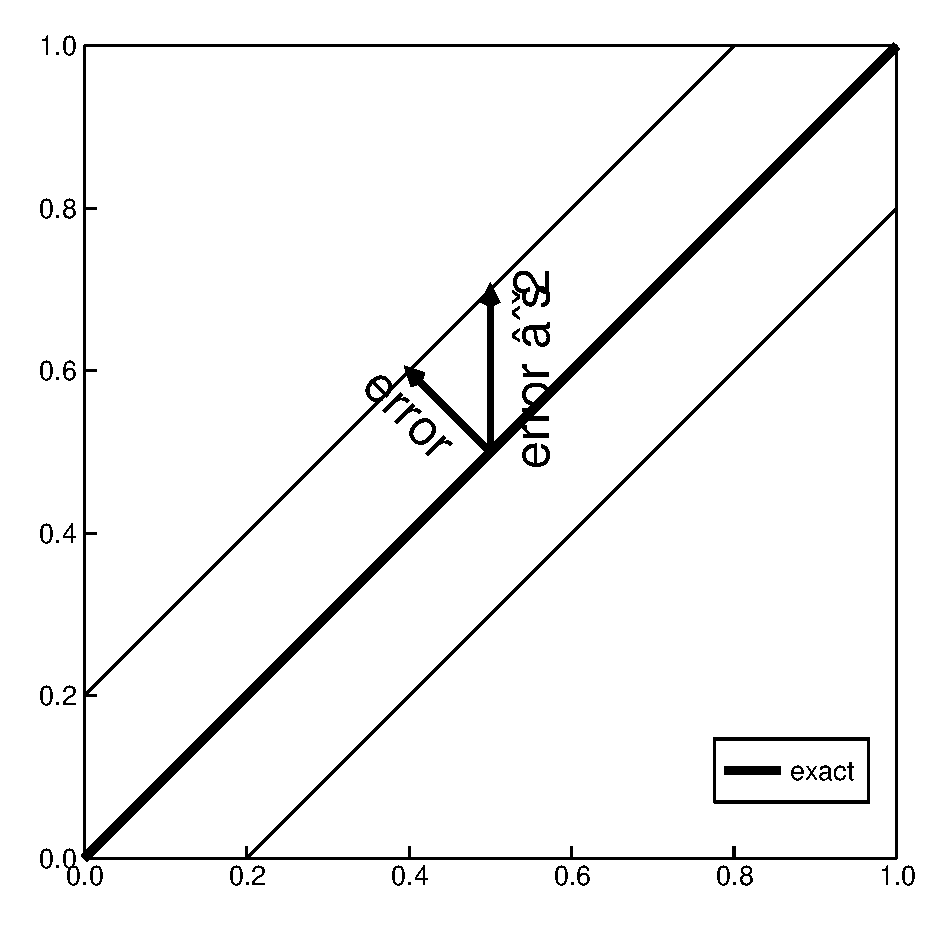
\includegraphics[width=0.5\textwidth]{figures/diagramdelta01.pdf}
\caption{The surface $y_1=y_2$ and the approximation to its measure by
  $\epsilon$-width characteristic functions. Using the original coordinates
  we perform an error of $\sqrt{2}$, but using the $y,Y$ coordinates
  we arrive to the correct expresion. Using the MonteCarlo Numerics, this
  error is dificult to detect, because both the numeric and the wrongly solved
  analityc formula have the same multiplicative mistake. Is only when we plug this into
Machta Zwanzig Formula that the error becomes evident. }\label{DiagramaDelta01}
\end{figure}

The simplest approach to this integral is using directly the expression in the $y$ and $Y$
coordinates, since the surface is orthogonal to the $Y$ axis:
  \begin{align} 
    \frac{A_\text{hopp}}{8} & = \iiiint \limits_
      {\substack{x, X, Y=0 \\ y=b\sqrt{2}}}^
               {\substack{x=a\sqrt{2}, y=b\sqrt{2} \\
                   X=a\sqrt{2}-x, Y =b \sqrt{2}-y }}
                \mkern-36mu
     \rd x   \rd y  \rd X   \rd Y
     \indicator{x^2+y^2 \geq 2 r^2} \delta (y)
     \label{pasoraro}
     \\   
     &=  \iint \limits_{x=0, y=-b\sqrt{2}}^{x=a\sqrt{2}, y=\sqrt{2}}
    \mkern-18mu  \rd x \rd y 
    (a\sqrt{2}-x)(b\sqrt{2}-y)
    \indicator{x^2+y^2 \geq 2 r^2} \delta (y)
    \\
    &= \int \limits _0^{a\sqrt{2}} \rd x
    b\sqrt{2} (a\sqrt{2}-x)
    \indicator{x^2\geq 2 r^2}
    \\
    &= \int\limits_{r\sqrt{2}}^{a\sqrt{2}} \rd x
    (2ab-xb\sqrt{2})
    \\
    &=\biggl[2abx-\frac{x^2b}{\sqrt{2}} \biggr]_{r\sqrt{2}}^{a\sqrt{2}}\\
      A_\text{hopp}&=8\sqrt{2}b(a-r)^2
  \end{align}
  Note that in \eqref{pasoraro} we do not use symmetry in
  $y$, due to the Dirac delta.
  Here we have to apply the reasoning that was outlined in section \ref{knownfacts}.
  Given that this event can be realized in two ways which are
  distinguishable by their direction, it is as if the surface has two sides.
  Thus, we can incorporate a multiplicative factor of $s=2$ into this expression, or include it in the denominator of 
  the expression for the mean time.

  \subsubsection{Disc collisions}
  For other cross-section areas we proceed in a similar manner. 
  Disc collisions occur when $\sqrt{x^2 + y^2} = r \, \sqrt{2}$, giving
  \begin{equation}
    \frac{A_\text{col}}{16}  = \iiiint\limits_
         {x,X,y,Y=0}^
         {\substack{x=a\sqrt{2},\, X=a\sqrt{2}-x
             \\ y =  b\sqrt{2},\,  Y=b\sqrt{2}-y}}
         \mkern-18mu
    \rd x \rd X \rd y \rd Y
    \delta (\sqrt{x^2+y^2}-\sqrt{2}r)
  \end{equation}
  \begin{multline}
    \frac{A_\text{col}}{16}  = \iint \limits_{x,y=0}^
      {x=a\sqrt{2},\, y=b\sqrt{2}}
    \mkern-18mu \rd x \rd y 
    \bigl[ 2ab-\sqrt{2}(ay+bx)+xy \bigr] \\
    \times
    \delta (\sqrt{x^2+y^2}-\sqrt{2}r)\\
    \end{multline}
  We change to polar coordinates as we did in \ref{app:volcyl}:
  \begin{align}
    x^2+y^2 =: \rho^2 \\   \Rightarrow   \delta(\sqrt{x^2+y^2}-\sqrt{2}r) \rightarrow
    \delta(\rho-\sqrt{2}r)   
    \end{align}
  Then we continue straightforwardly:
  \begin{widetext}
    \begin{align}\label{app:colgeneral}
      A_\text{col}/16 & =\iint\limits_{\rho=0, \theta=\beta}^{\rho=r, \theta=\alpha}
      \mkern-18mu
    \rd \theta \rd \rho \rho
    \bigl[2ab-\sqrt{2}\rho(a\sin\theta+b\cos\theta)+\rho^2\cos\theta\sin\theta
      \bigr]
    \delta(\rho-\sqrt{2}r) \\
    &=\int_\beta^\alpha \rd \theta \sqrt{2}r
    \bigl[
      2ab-2r(a\sin\theta+b\cos\theta)+2r^2\cos\theta\sin\theta)
      \bigr] \\
    A_\text{col} & = 16\sqrt{2} \bigl( 2abr(\alpha-\beta)
    + 2r^2 [a (\cos \alpha-\cos\beta) -b (\sin\alpha -\sin\beta)]
     + r^3(\sin^2 \alpha -\sin^2\beta) \bigr)
    \end{align}
    \end{widetext}
    We have used the same trick as in previous subsection to obtain a general expression
    that works even when hopping is not possible.
    In the case of $r<w/4$ (all hopping possible)
    we have the substitution $\alpha=\pi/2$ and $b=0$,
    obtaining the result stated previously
    in eq. \ref{AreaChoque}. It is practical to leave here the expression for 1/4 of the
    total area. The symmetry of the cases makes it so that when the phase space splits
    into disjoint components, the volume accessible and the area accessible scale in
    the same manner.
    
    \subsubsection{Wall collisions}

    For a collision with the wall, the $x_i$ give suitable coordinates. Once again, we
    have to be careful with the multiplicative factors that appear due to change
    of variables. Let us suppose that we want the area that represents hits of
    the disc 2 against the right wall. That means that $x_2-a=0$. 
    \begin{multline}
      A_{x_2=a}  =\iiiint \limits_{-a,-a,-b,-b}^{a,a,b,b}
       \mkern-9mu \rd x_1 \rd x_2 \rd y_1 \rd y_2 
       \indicator{(x_1-x_2)^2+(y_1-y_2)^2 \geq (2 r)^2}
       \\ \times \delta (x_2-a)\\
      =\iiint\limits _{-a,-b,-b}^{a,b,b} \rd x_1  \rd y_1 \rd y_2 
      \indicator{(x_1-a)^2+(y_1-y_2)^2 \geq (2 r)^2} 
    \end{multline}
    Changing variables;
    \begin{equation}
      \frac{y_1-y_y}{\sqrt{2}} =  y  \qquad \frac{y_1+y_y}{\sqrt{2}}=Y \qquad \frac{x_1-a}{\sqrt{2}}=x
    \end{equation}
    Integrating over $x$,
    \begin{align}\label{areachoquexy}
      A_{x_2=a} & =\sqrt{2} \mkern-18mu
      \iiint \limits
      _{-\sqrt{2}a,-\sqrt{2}b,-\sqrt{2}b+|y]}^{0,\sqrt{2}b,\sqrt{2}b-|y|}
        \mkern-18mu \rd x \rd y \rd Y 
        \indicator{(x^2+y^2 \geq 2 r^2}
        \\
        &=2\sqrt{2}\mkern-9mu
        \iint \limits_{-\sqrt{2}a,-\sqrt{2}b}^{0,\sqrt{2}b}
        \mkern-9mu
        \rd x \rd y (\sqrt{2} b - |y|)
      \indicator{(x^2+y^2 \geq 2 r^2}
    \end{align}
    
    
    In the case that all hopping is possible there are no problems with the above derivations,
    but if vertical hopping is excluded then there are differences.
 If $r>h/4$, and disc 2 starts
    on the left, it will never be able to hit the right wall. So, actually, this
    is a subsystem of the whole  system in which our general formula needs
    to be adjusted. 
%    We can trace this problem to the original purpose of
%    \eqref{meanfreetime}, namely to
%    find mean escape times. A particle cannot escape a volume if the exit is
%    not in contact with that volume. So after hopping in one or both direction
%    becomes impossible, the dynamical system gets split into disjoint components
%    that never mix under the dynamics (ergodic components). 
%So we have to take that
%    into account. 
    When $h/4<r<w/4$, a disk cannot interchange left--right positions,
    but can still move across all vertical available space.  After $r\geq w/4$,
    the system gets split again into two more disjoint components.
    So, when we calculate the available volume, we use only the
    part of the volume corresponding to the set where the event can occur
%    In this particular case, it is
%    if as the volume gets split into disjoint components, namely 1,2 or 4 of the
%    total avaible. This can be seen in the numerics as a discontinuity both
%    in  the simulated data and in the exact expression. The avaible area
%    for this event remains the same. 
    
    Again, it is simpler to evaluate the last expression in eq. \ref{areachoquexy}
    in the excluded space and then to subtract that from the whole configuration
    space evaluation:

    \begin{widetext}
    \begin{align}
      A_{x_2=a} & =4\sqrt{2}\iint \limits_{0,0}^{\sqrt{2}a,\sqrt{2}b}
        \rd x \rd y (\sqrt{2} b - y)
        \indicator{(x^2+y^2) \geq 2 r^2}\\
     &=\underbrace{4\sqrt{2}\iint \limits _{0,0}^{\sqrt{2}a,\sqrt{2}b}
        \rd x \rd y (\sqrt{2} b - y)}_{\text{whole space}}
        -\underbrace{
          4\sqrt{2}\iint \limits_{0,0}^{\sqrt{2}a,\sqrt{2}b}
        \rd x \rd y \rd Y 
        \indicator{(x^2+y^2) < 2 r^2}(\sqrt{2} b - y)}_{\text{excluded space}}
    \end{align}
    \end{widetext}
    The integrals are again routine to evaluate: the whole space part
    gives
    \begin{equation}
      \frac{1}{4}A_{\text{whole}}=8ab^2.
    \end{equation}
    For the excluded part, we perform the same routine of evaluating the circular region
    in polar coordinates and the triangular regions, if they exist, in Cartesian coordinates.
    From the circular sector we get (see Fig.~\ref{CasosIntegra} and the following explanation
    for $\alpha, \beta$ variables):
    \begin{equation}
      A_{sector}=8 b r^2(\alpha-\beta)+16r^3/3(\cos\alpha - \cos\beta)
    \end{equation}
    The upper triangle where to give, for $\alpha < \pi/2$,
    \begin{equation}
    A_{ut}=\frac{8}{3}b^2\sqrt{r^2-b^2}
    \end{equation}
    And the lower triangle a similar expression with $a$ instead of $b$.

%    Now, these are actually all the expressions needed for any collision, but
%    to combine them and to use them meaningfully is still needed. For example,
%    this last calculated area could be used as representation of the event of
%    the disc 1 hitting the right wall, or the disc 2 hitting the left wall. Both
%    can make sense in the case of excluded horizontal interchange. What would be
%    the expression of any disk hitting the right wall? It would be twice this expression
%    but only before the exclusion sets in. Then we need to take into account
%    the disjointedness of the phase space and divide the cases accordingly.

%    In the same vein we could conclude that the area that represents
%    any collision (wall, discs, etc) can be obtained by summing all the other
%    areas, before hopping is excluded. If there is some sort of hindrance to
%    the movement, then the expression becomes different, again, a sum over
%    disjoint components. This could lead to tedious exercises in cases ramifications.

\section{Numerical method for calculating surface area}
    
All code used for the simulations is available, in keeping with the philosophy of open science.

For simplicity, we used traditional rejection sampling to calculate the free volume and cross-sectional areas.

The cross-sectional areas are calculated by fattening the surface $g(\mathbf{x}) = 0$ to $S_\epsilon := \{ \mathbf{x} : 0 \le g(\mathbf{x}) \le \epsilon \}$, or in the
case of the hopping cross-section $S_{2 \epsilon} := \{ \mathbf{x}: \|g(\mathbf{x}) \| \le \epsilon \}$.

Thus 
$$A = \lim_{\epsilon \to 0} \frac{ \int \mathbf{1}_{S_\epsilon}}{\epsilon}$$ 
is calculated by sampling points from the whole volume and rejecting those lying outside $S_\epsilon$.
 
As in the analytical calculation, the width of this strip must be calculated correctly by dividing by $\| \nabla g(x) \|$.

    
\section*{Acknowledgements}


DPS thanks Sidney Redner for posing the question that led to this work, and the Marcos Moshinsky Foundation for financial support via a fellowship.
Support is also acknowledged from grants CONACYT-Mexico CB-101246 and CB-101997, and DGAPA-UNAM PAPIIT IN117117.




\bibliography{TwoDiskBiblio}



\end{document}
